%
% This file is part of Calicut University Question Paper Collection.
%
% Copyright (c) 2012-2015 Mohammed Sadik P. K. <sadiq (at) sadiqpk (d0t) org>.
% License: GNU GPLv3 or later
%
% Calicut University Question Paper Collection is free software: you can
% redistribute it and/or modify
% it under the terms of the GNU General Public License as published by
% the Free Software Foundation, either version 3 of the License, or
% (at your option) any later version.
% 
% Calicut University Question Paper Collection is distributed in the hope
% that it will be useful,
% but WITHOUT ANY WARRANTY; without even the implied warranty of
% MERCHANTABILITY or FITNESS FOR A PARTICULAR PURPOSE.  See the
% GNU General Public License for more details.
% 
% You should have received a copy of the GNU General Public License
% along with Calicut University Question Paper Collection.
% If not, see <http://www.gnu.org/licenses/>.
% 
%

%% NOT INCLUDED due to many errors in the question paper

%% \def \subj{AI 09 306---ELECTRIC CIRCUITS AND NETWORK THEORY}

%% \mainhead{D 20632}{2}
%% \semthree{OCTOBER 2011}
%% \sub{\subj}
%% \maxtime

%% \partA

%% \iitem State superposition theorem.
%% \item Define the terms impedance and admittance.
%% \item State the significance of final value theorem.
%% \item Define propagation constant.
%% \item Name an application each for band elimination filter and attenuator.

%% \markA
%% \partB

%% \item State and prove any four properties of Laplace transform.
%% \item Write notes on Blode plot.
%% \item Find the Laplace transform of a full wave rectified sinusoidal signal.
%% \item State the restrictions on pole and zero location in transfer functions.
%% \item Define and state the significance of various ABCD parameters.
%% \item For a given, Z$_{11} = 3 \Omega$, Z$_{12} = 3 \Omega$, Z$_{21} = 3 \Omega$ and
%%   Z$_{22} = 3 \Omega$, find the admittance matrix.

%% \markB
%% \partC

%% \item \iitem For the following circuit, find the current in the 15$\Omega$ resistor when the switch
%%   is closed at $t = 0$. Assume that the initial current through the inductor is zero.
%% \Or

%% \newpage \again

%% \item Sine wave is applied to the following circuit when the switch S is closed at $t = 0$.
%%   Find the current $i(t)$.
%% \ene

%% \item \iitem For the following network, find the transfer functions and driving port impedance
%% \item Draw the pole zero diagram for the given network function and hence find 
%% \ene
%% \Or
%% \item \iitem \iitem  Find the transmission parameters for the following circuit:
%% \item Design a T type attenuator to give an attenuation of 65 dB to work in a line of 600 impedance.
%% \ene\ene

%% \item \iitem Find the Z parameter of the following circuit:

%% \begin{figure}[!h]
%%   \centering
%%   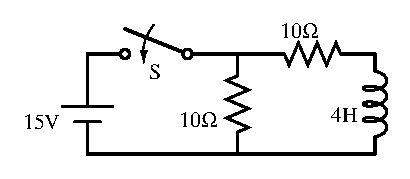
\includegraphics{src/s3/ai/09_306/fig001}
%% \end{figure}
%% \Or
%% \item Design a symmetrical bridged-T attenuator with an attenuation of 30 dB and terminated into a load of 600
%% \ene

%% \item \iitem \iitem Design a low pass filter in both T and configurations with a cut-off frequency
%%   of 2kHz when terminated with resistance.
%% \item Discuss the Butterworth filter characteristics.
%% \ene 
%% \Or
%% \item Derive the expression for the cut-off frequency of a constant high pass filter and
%%   discuss its characteristics.
%% \ene
%% \ene
%% \markC
     

